\documentclass[conference]{IEEEtran}
\usepackage[pdftex]{graphicx}
\usepackage{amsmath}
\usepackage{multirow}
\usepackage{hyperref}

\begin{document}
	
\title{Dynamic Region-biased \\ Rapidly-exploring Random Trees for \\ Motion Planning in Cluttered Workspaces}

\author{\IEEEauthorblockN{Ryan Gibson}
\IEEEauthorblockA{Department of Computer Science\\
University of North Carolina at Chapel Hill\\
Chapel Hill, NC 27599}}

\maketitle
\IEEEpeerreviewmaketitle

\section{Introduction}

Many current motion planners employ sampling-based strategies in order to explore the workspace and rapidly construct valid paths between source and goal configurations. Such methods have proven to be successful in practice, but still face poor performance in cluttered workspaces that include ``narrow passages'' (spaces in which sampling a valid configuration is very low).

In this paper, we explore a strategy for using a topological representation of the free workspace to guide random sampling. This will allow for the dynamic manipulation of sampling regions through the workspace in order to more easily find potential paths through narrow passages.

\section{Related Work}

Denny et al. \cite{DRRRT} proposed a strategy to use a Reeb Graph as a topological representation of the free workspace. This ``embedding graph'' is relatively easy to compute (see the algorithm in \cite{ReebGraphs}) and is used to guide the growth of a Rapidly-exploring Random Tree (RRT). Much of this paper is adapted from this strategy.

\section{Problem Definition}

Here, we focus on the holonomic motion planning problem.\footnote{The authors of \cite{DRRRT} show that their method can be easily extended to nonholonomic robots.} That is, we are concerned with robots in which every degree of freedom is fully and independently controllable. These degrees of freedom (DOFs) characterize the movement of the robot in its 2-d or 3-d workspace.

We now formalize this problem. We take as input the geometric description of the robot's environment $e$ (e.g. lists of vertices in 2-d or 3-d that represent polyhedral obstacles), a starting configuration $q_s$, and a goal configuration $q_g$. Each of these configurations is a single parameterization of the DOFs of the robot $q = \langle x_1, \dots, x_n \rangle$ and is considered ``valid'' if a robot placed at $q$ does not collide with itself or the environment geometry. Such a collision check is implemented by a \texttt{Clear} algorithm.

Then, the goal is to output a continuous sequence of valid configurations from $q_s$ to $q_g$. This describes a trajectory that the robot can follow in order to complete the motion planning problem at hand.

\section{Methods}

Following \cite{DRRRT}, we first precompute a Reeb Graph in the environment of interest. This is a topoplogical structure that represents the entire free workspace (and its topology so that the homotopy classes of paths can be determined). An example of such a graph in one of our environments is shown in \autoref{fig:reeb_graph_example}.

\begin{figure}[h]
	\centering
	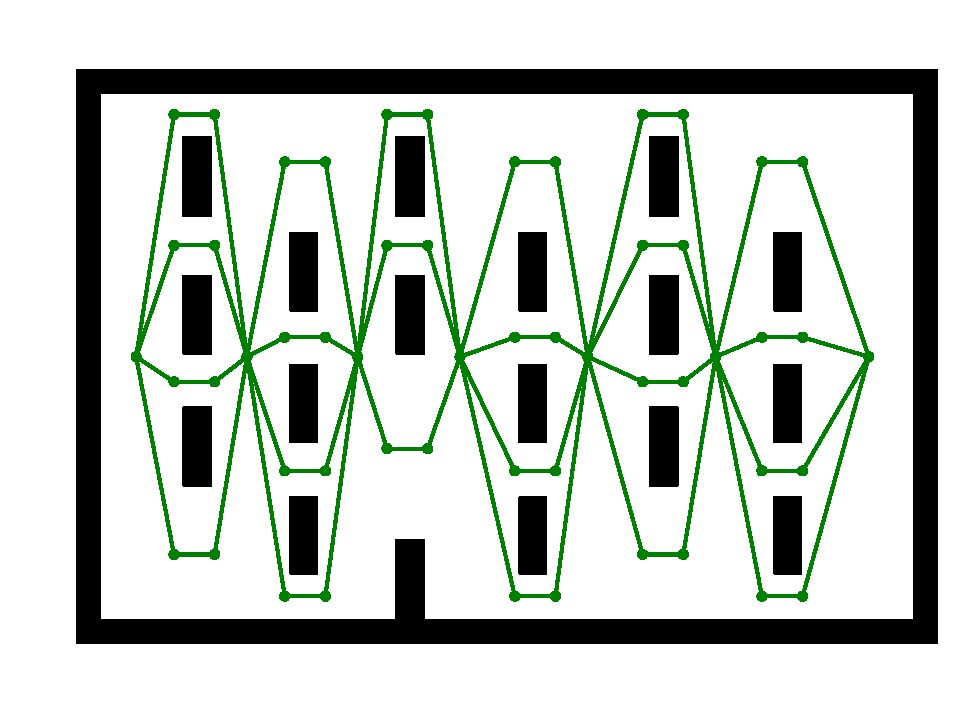
\includegraphics[width=1.72in]{figures/partial_reeb_graph_example.pdf}
	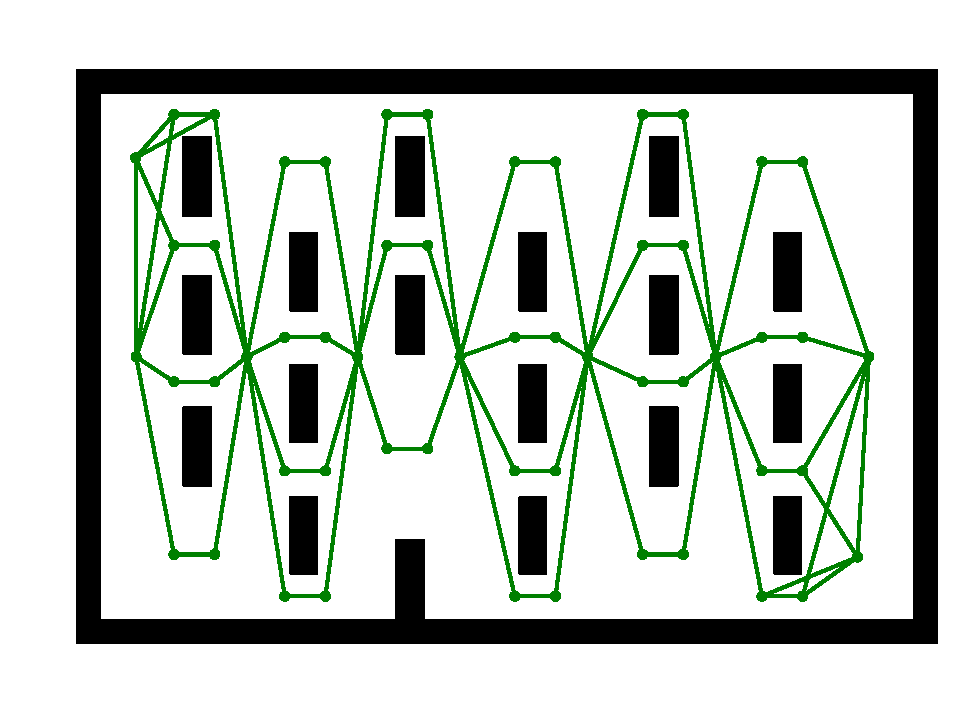
\includegraphics[width=1.72in]{figures/full_reeb_graph_example.pdf}
	\caption{Left: Example Reeb Graph of our ``Barriers'' environment. Right: Example Reeb Graph after source and goal configurations are added and connected.}
	\label{fig:reeb_graph_example}
\end{figure}

Then, given a query involving a start configuration $q_s$ and goal configuration $q_g$, we connect these configurations to nearby nodes in the Reeb Graph and make its edges directed so that all paths point from $q_s$ to $q_g$. Additionally, we prune paths that never reach $q_s$. This forms a directed ``Flow Graph'' through the workspace.

Using this, we create a sampling region at the source configuration $q_s$ and advance the region along the edges of the Flow Graph. These sampling regions split into multiple, independently moving regions when they reach nodes with out-degree greater than one. Similarly, regions are merged at nodes with in-degree greater than one.

In this way, we may have many different sampling regions at any given time. Hence, when sampling a new configuration in our space, we first choose a random region, sample a configuration from that region, and advance the region along its edge in the Flow Graph. This grows our Rapidly-exploring Random Tree along the edges of the Flow Graph until the goal configuration $q_g$ is reached. We visualize this process in \autoref{fig:region_splitting}.

\begin{figure}[h]
	\centering
	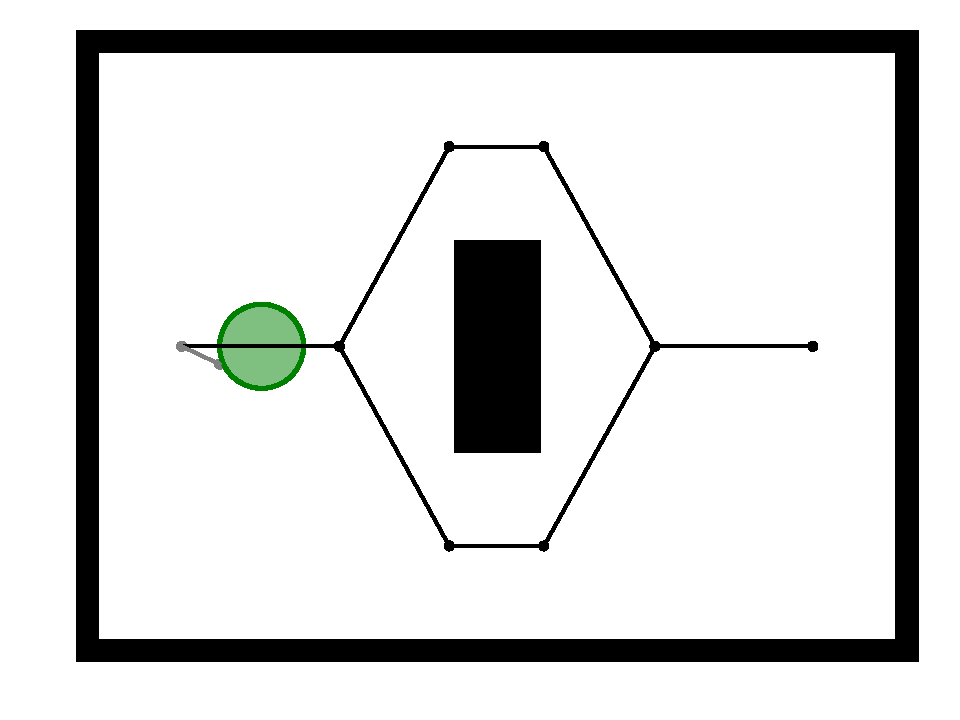
\includegraphics[width=1.72in]{figures/split1.pdf}
	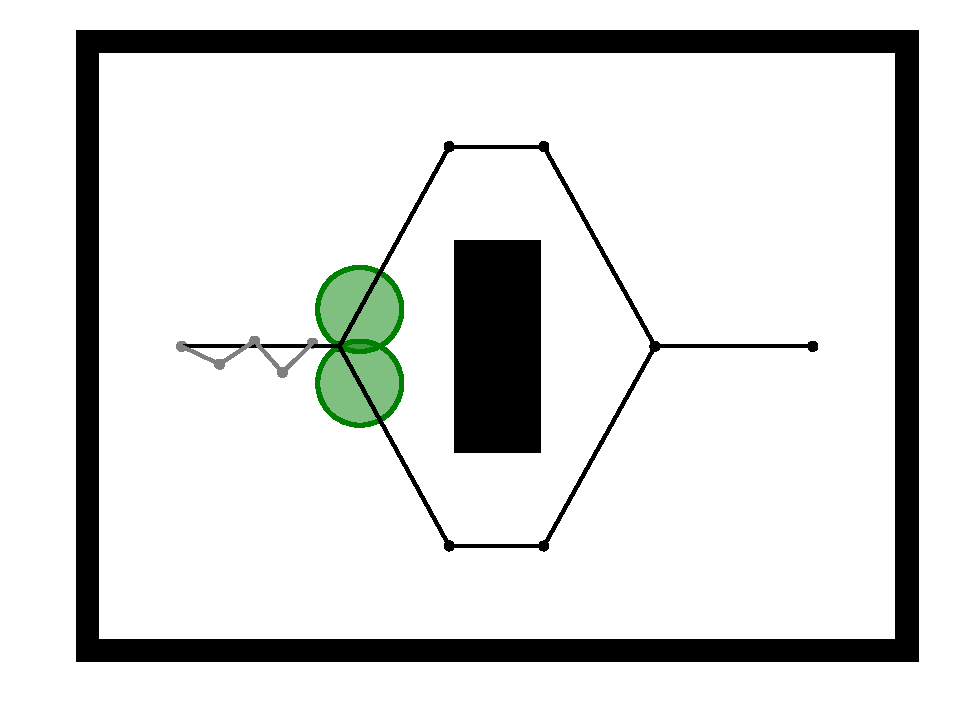
\includegraphics[width=1.72in]{figures/split2.pdf}
	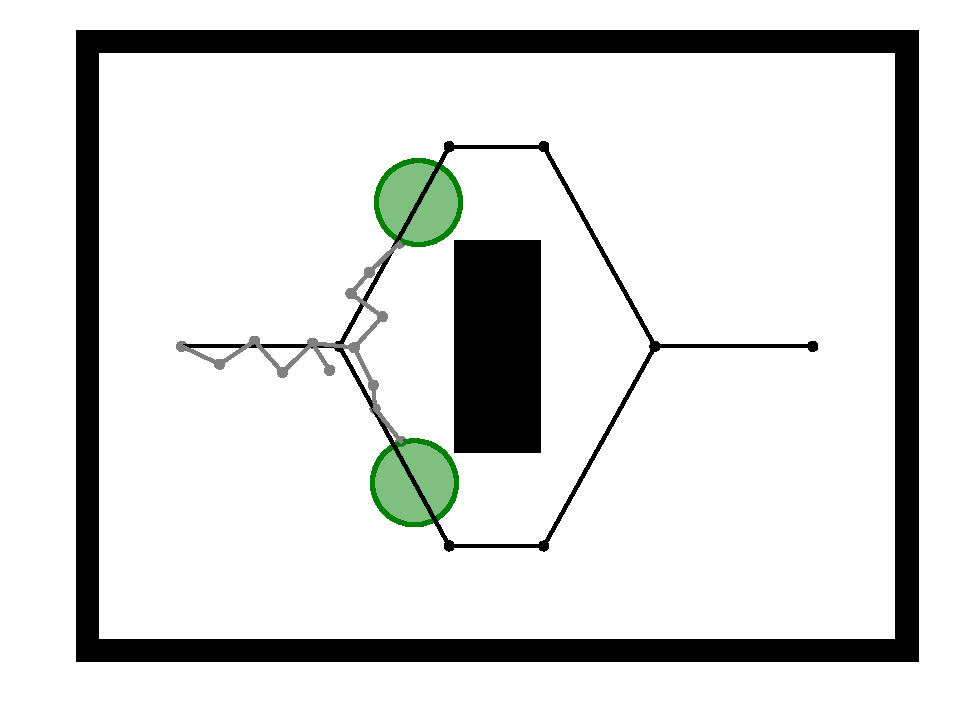
\includegraphics[width=1.72in]{figures/split3.pdf}
	\caption{Example growth of a DRRRT as the sampling regions split. Top Left: Start of tree growth with one region. Top Right: Sampling region splits into two at a node in the Flow Graph. Bottom: DRRRT growth continues, choosing randomly between available sampling regions on each iteration.}
	\label{fig:region_splitting}
\end{figure}

Optionally, one can abandon sampling regions if they repeatedly fail to yield valid sampled configurations (``as [this] likely [represents] a path that is only viable for [the] workspace and not for the robot's [configuration space]'' \cite{DRRRT}). We do not take this approach, but it may be useful in some environments.

To retain the property of probabilistic completeness, one can also consider the entire workspace to be one large sampling region. In essence, this resorts to standard RRT growth with probability $1 / (\text{current number of sampling regions})$.

\section{Results}

We implemented both the standard RRT and DRRRT methods as discussed above in a custom simulator. Then, we repeatedly ran both motion planning strategies on the five environments shown in \autoref{fig:problem_environments}.

\begin{figure}[h]
	\centering
	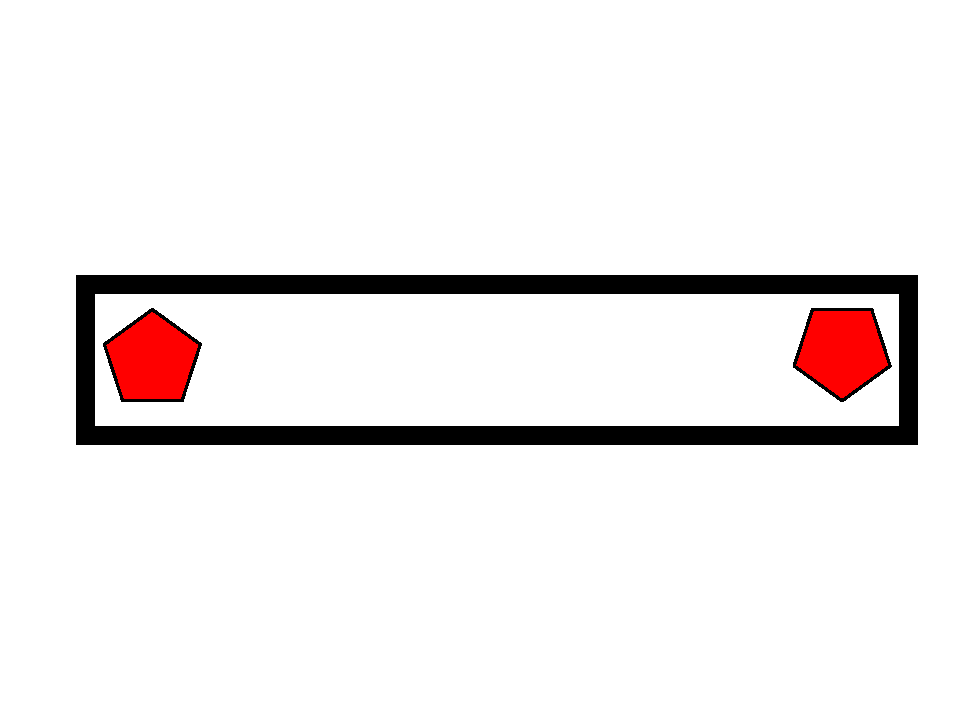
\includegraphics[clip, trim=0cm 4cm 0cm 4cm, width=2.5in]{figures/hallway_problem.pdf}\\
	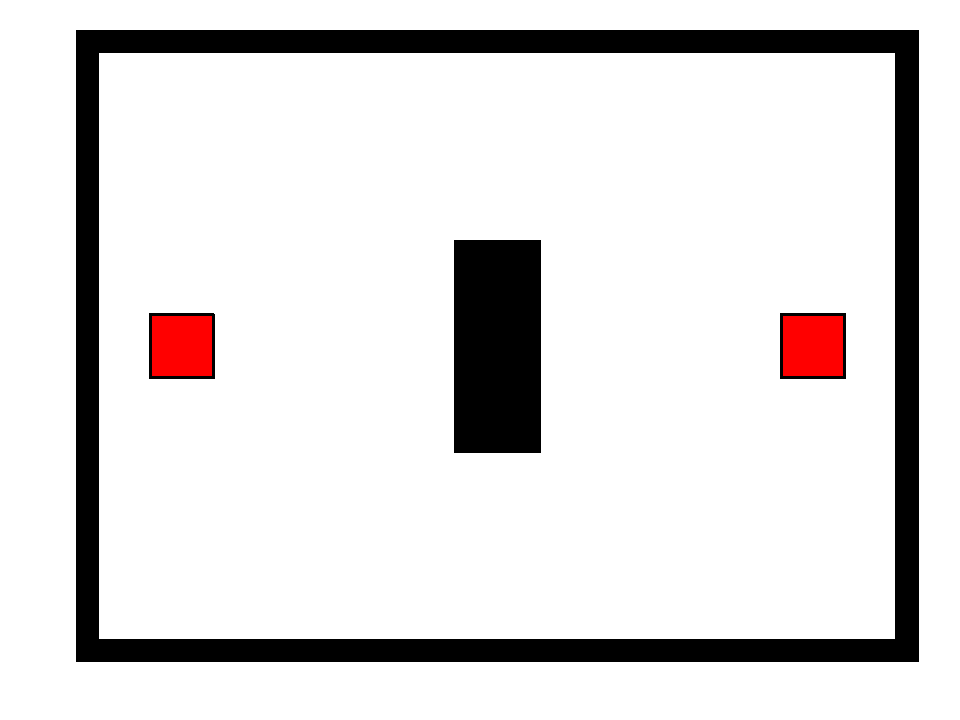
\includegraphics[width=1.72in]{figures/split_problem.pdf}
	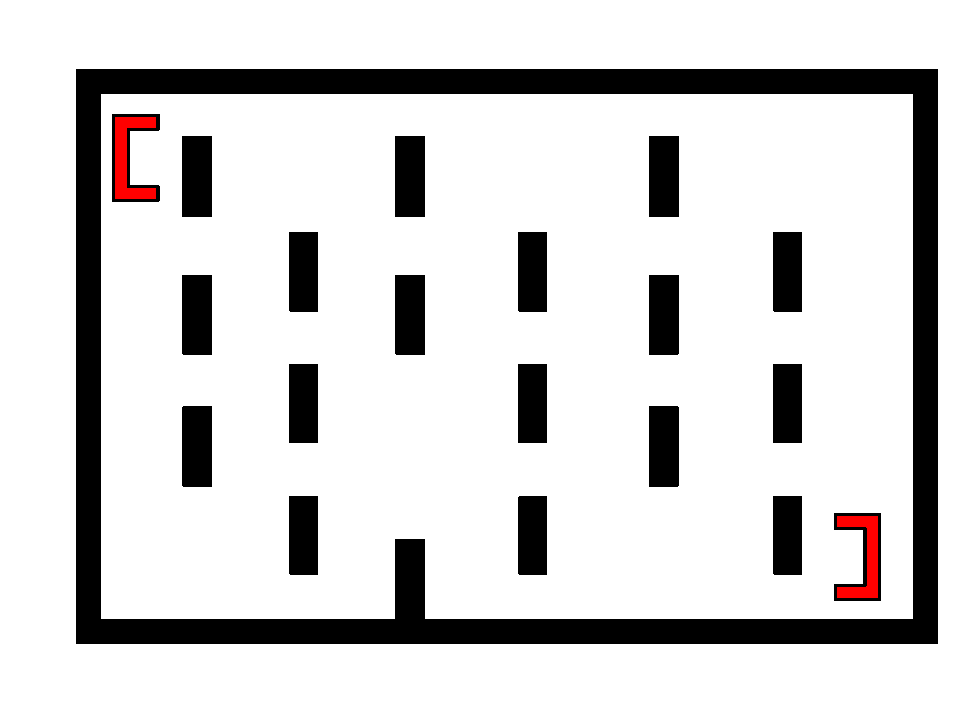
\includegraphics[width=1.72in]{figures/barriers_problem.pdf}
	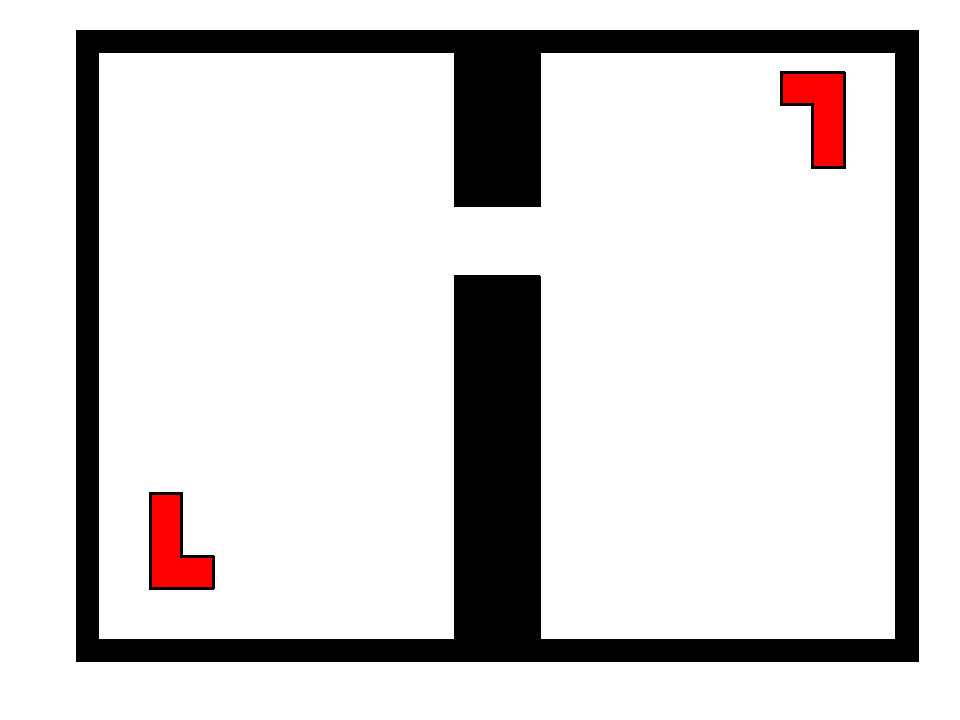
\includegraphics[width=1.72in]{figures/narrow_problem.pdf}
	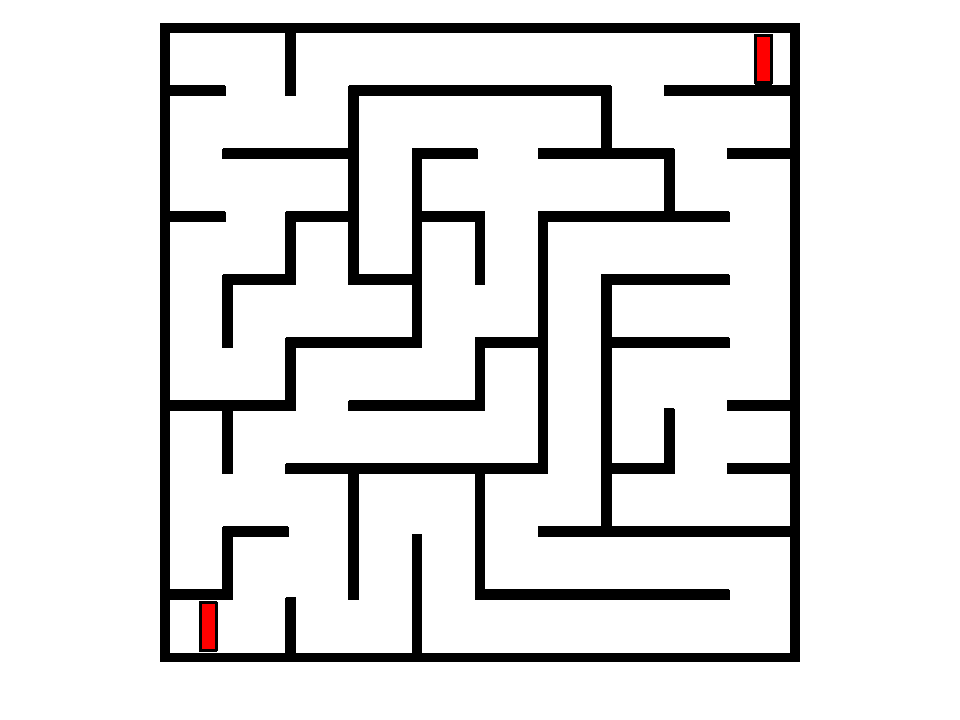
\includegraphics[width=1.72in]{figures/maze_problem.pdf}
	\caption{Our five testing environments, with source and goal configurations shown in red (in all cases, the source is on the left and the goal is on the right). Top-to-Bottom, Left-to-Right: ``Hallway'', ``Split'', ``Barriers'', ``Narrow'', ``Maze''.}
	\label{fig:problem_environments}
\end{figure}

In particular, we ran RRT and DRRRT motion planning 1000 times on each environment and have summarized the observed performance in \autoref{fig:results_table}.

In all trials, we grow the RRT/DRRRT by nodes no further away than 2.5\% of the environment's width from the nearest neighbor in the tree. Each such tree growth succeeds only if all configurations between the parent and children nodes are valid, checked with a step size of 0.5\% of the environment's width. These choices are somewhat arbitrary, but importantly, are the same in both the experiments using the standard RRT and those using our DRRRT strategy.

\begin{figure}[h]
	\centering
	\begin{tabular}{|c||c|c|c||}
		\hline\multirow{2}{*}{Planner}&\multicolumn{3}{|c||}{RRT}\\
		\cline{2-4}&Success Rate&Nodes&\texttt{Clear} calls\\\hline
		Hallway&100\%&62&532\\
		Split&100\%&443&2.7K\\
		Barriers&83\%&660&16.9K\\\
		Narrow&45\%&1150&11.5K\\
		Maze&0\%&*&*\\\hline\hline
		\multirow{2}{*}{Planner}&\multicolumn{3}{|c||}{DRRRT}\\
		\cline{2-4}&Success Rate&Nodes&\texttt{Clear} calls\\\hline
		Hallway&100\%&47&231\\
		Split&100\%&90&450\\
		Barriers&100\%&326&12.5K\\
		Narrow&82\%&72&5.2K\\
		Maze&100\%&171&1288\\\hline
	\end{tabular}
	\caption{Success rates, average number of tree nodes, and average number of \texttt{Clear} calls for RRT and DRRRT motion planning in our five environments. Results are averaged over 1000 trials, only including runs that found a valid path before calling \texttt{Clear} 25K times.}
	\label{fig:results_table}
\end{figure}

Across all of our environments, DRRRT obtains a significant improvement in all measured metrics: success rate, number of nodes added to the tree before a valid path is found, and number of \texttt{Clear} calls needed to find a valid path.

We would like to note that the ``Barriers'' environment involves the repeated splitting of DRRRT sampling regions across many available workspace paths (see the Reeb Graph in \autoref{fig:reeb_graph_example}). In this way, our method is ``forced'' to explore many different narrow passages in the workspace rather than proceeding directly to the goal along a single path. However, even in this near-worst-case scenario, DRRRT performs better than RRT by a considerable margin.

We also plot boxplots in \autoref{fig:results_boxplots} of the number of collision checks needed before a valid path is found in these experiments. Here (since collision checking is one of the more computationally intensive parts of motion planning), we find that DRRRT is not only faster than RRT on average, but is also more consistent (i.e. less stochastic with respect to runtime) in many cases.

Of course, the DRRRT method requires the precomputation of the environment's embedding graph, but we have found that this accounts for a surprisingly small fraction of the time required for the entire motion planning pipeline.

As such, the dynamic region-biased variant should be preferred over standard RRT growth strategies if a robot's movements through its environment are expected to adhere to valid paths in the workspace and an embedding graph is feasible to compute.

\begin{figure}[h]
	\centering
	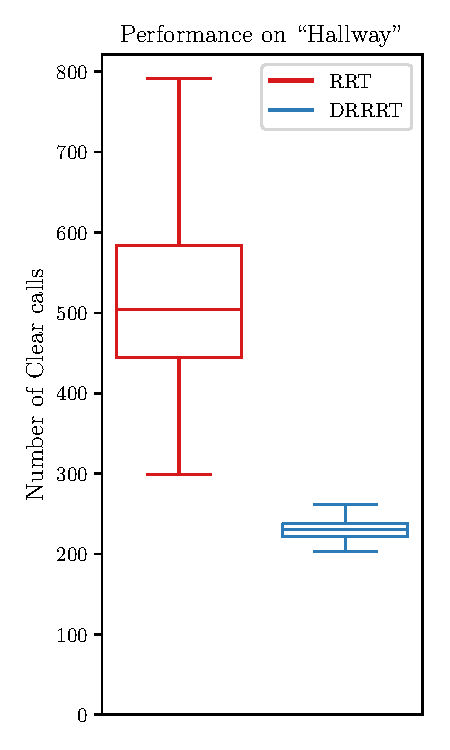
\includegraphics[width=4.3cm]{figures/hallway_boxplot.pdf}
	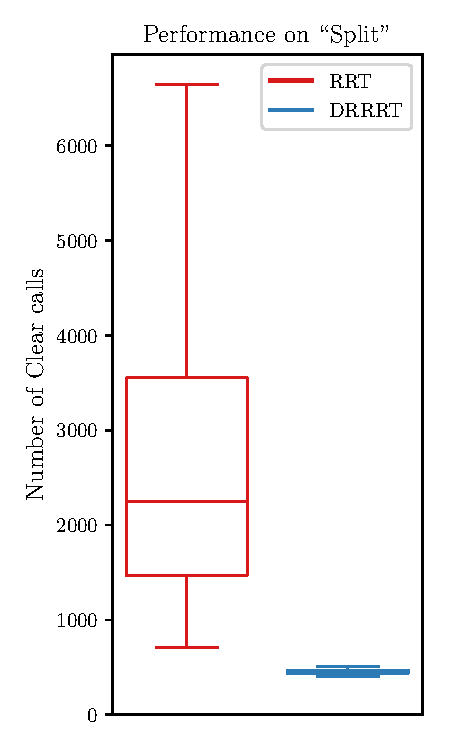
\includegraphics[width=4.3cm]{figures/split_boxplot.pdf}
	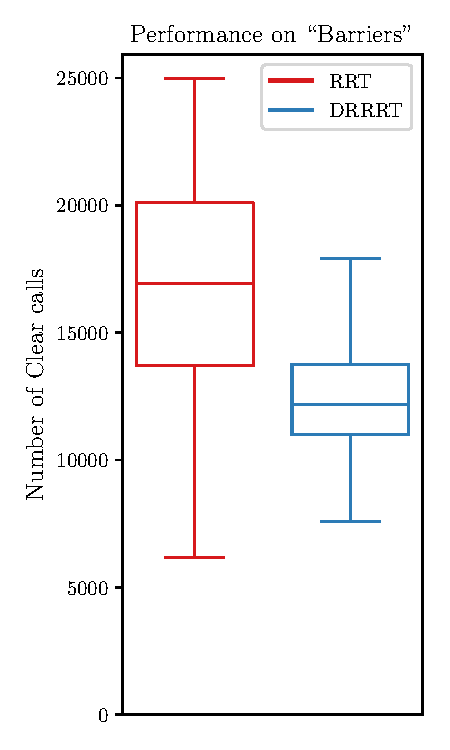
\includegraphics[width=4.3cm]{figures/barriers_boxplot.pdf}
	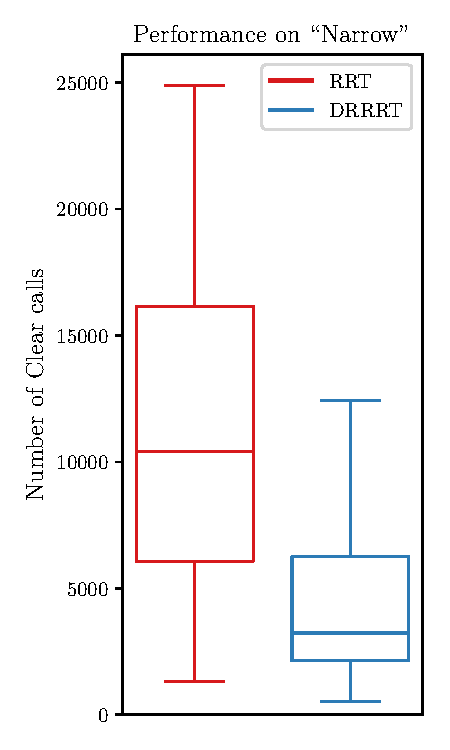
\includegraphics[width=4.3cm]{figures/narrow_boxplot.pdf}
	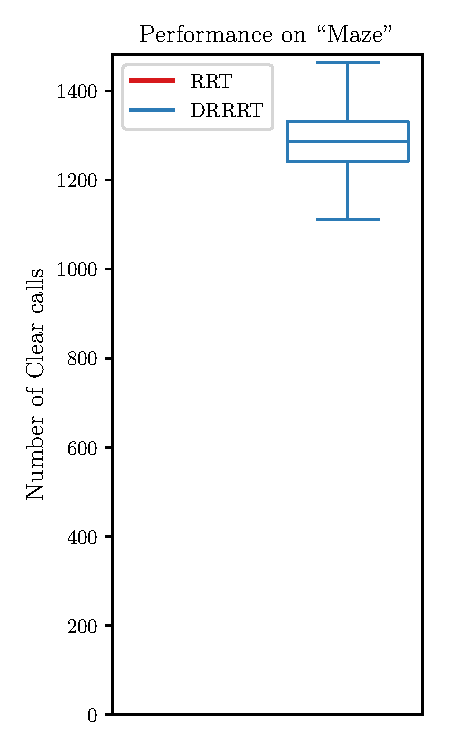
\includegraphics[width=4.3cm]{figures/maze_boxplot.pdf}
	\caption{Boxplots of the number of \texttt{Clear} calls required in our experiments before a valid path was found. Here, only the results for successful motion planning runs are included. Note that no boxplot is shown for the standard RRT growth on the ``Maze'' environment since this never succeeded in our trials.}
	\label{fig:results_boxplots}
\end{figure}

\section{Conclusion and Future Work}

In this paper, we analyzed the effectiveness of a dynamic region-based variant of RRT in motion planning problems. In our test cases, we found that this variant provides a significant improvement over the standard RRT.

In particular, DRRRT was able to succeed more often than RRT, ran much more quickly than RRT, and was more consistent than RRT in the number of collision checks required before a valid path was found.

Following the approach of \cite{DRRRT}, we chose to use a Reeb Graph as our embedding graph to guide tree growth. However, this choice is arbitrary and any graph that sufficiently captures the topology of the workspace could be used. As such, future work should consider using different graph structures for this purpose.

Notably, our work here depends on the precomputation of the embedding graph, which may not be tractable in environments with dynamic obstacles. Future work should focus on extending this strategy to situations in which obstacles deform or move as time progresses.

Indeed, the original description of Reeb Graph computation in \cite{ReebGraphs} provides an online algorithm (i.e. it is provided the environment mesh triangles one at a time and computes the graph piece-by-piece) which could be used to update the portions of the graph that correspond to dynamic obstacles, thus allowing our method to be used in dynamic situations.

Lastly, the method as presented here depends heavily on valid paths through the configuration space corresponding to valid paths through the workspace. For some applications, this may not be the case and additional work should focus on if our strategy can be adapted to work in such situations.

\section*{Acknowledgment}

We would like to thank the authors of OMPL for the work on their comprehensive motion planning library. Our ``Barriers'' and ``Maze'' environments are based on their ``Barriers'' and ``UniqueSolutionMaze'' 2D problem configurations, respectively.

We would also like to thank Ron Alterovitz for his feedback on drafts of this paper and guidance through the general robotics literature.

\begin{thebibliography}{2}
\bibitem{DRRRT}
Jory Denny, Read Sandstrom, Andrew Bregger, Nancy M. Amato, ``Dynamic Region-biased Rapidly-exploring Random Trees.'' \emph{The Workshop on the Algorithmic Foundations of Robotics} (2016).
\bibitem{ReebGraphs}
Valerio Pascucci, Giorgio Scorzelli, Peer-Timo Bremer and Ajith Mascarenhas. ``Robust On-Line Computation of Reeb Graphs: Simplicity and Speed.'' \emph{ACM SIGGRAPH} (2007).
\end{thebibliography}

\end{document}


